\chapter{A 25-body Example}

\section{A $25$-body run}

\abc

\bob
Time to start a real experiment!  This will be our first chance to put
our {\st nbody\_sh1.C} engine to good use.  I remember that we had a
number of options built in, but for simplicity, let us just use the
default settings.

\carol
Fine.  Let's see. that means letting the system run for 10 time units,
with energy diagnostics being output every time unit, and all that
with a standard step size control parameter of 0.03.

\cba

\begin{small}
\begin{verbatim}
|gravity> sphere -n 25 | ../chap8/nbody_sh1 > s25.out
seed = 1063318557
Starting a Hermite integration for a 25-body system,
  from time t = 0 with time step control parameter dt_param = 0.03  until time 10 ,
  with diagnostics output interval dt_dia = 1,
  and snapshot output interval dt_out = 1.
at time t = 0 , after 0 steps :
  E_kin = 0 , E_pot = -0.571622 , E_tot = -0.571622
                absolute energy error: E_tot - E_init = 0
                relative energy error: (E_tot - E_init) / E_init = -0
at time t = 1.00026 , after 4154 steps :
  E_kin = 1.57024 , E_pot = -2.14216 , E_tot = -0.571911
                absolute energy error: E_tot - E_init = -0.000289307
                relative energy error: (E_tot - E_init) / E_init = 0.000506117
at time t = 2.00002 , after 15063 steps :
  E_kin = 0.574657 , E_pot = -1.14657 , E_tot = -0.571912
                absolute energy error: E_tot - E_init = -0.000289794
                relative energy error: (E_tot - E_init) / E_init = 0.000506968
at time t = 3.00001 , after 24785 steps :
  E_kin = 0.735507 , E_pot = -1.30742 , E_tot = -0.571913
                absolute energy error: E_tot - E_init = -0.000290734
                relative energy error: (E_tot - E_init) / E_init = 0.000508612
at time t = 4.00002 , after 37188 steps :
  E_kin = 1.1189 , E_pot = -1.69081 , E_tot = -0.571914
                absolute energy error: E_tot - E_init = -0.000291627
                relative energy error: (E_tot - E_init) / E_init = 0.000510175
at time t = 5.00002 , after 60274 steps :
  E_kin = 1.07524 , E_pot = -1.64716 , E_tot = -0.571917
                absolute energy error: E_tot - E_init = -0.000294566
                relative energy error: (E_tot - E_init) / E_init = 0.000515317
at time t = 6 , after 109752 steps :
  E_kin = 1.68677 , E_pot = -2.25869 , E_tot = -0.571926
                absolute energy error: E_tot - E_init = -0.000304007
                relative energy error: (E_tot - E_init) / E_init = 0.000531832
at time t = 7 , after 445974 steps :
  E_kin = 1.9559 , E_pot = -2.52792 , E_tot = -0.572019
                absolute energy error: E_tot - E_init = -0.000396555
                relative energy error: (E_tot - E_init) / E_init = 0.000693737
at time t = 8 , after 805101 steps :
  E_kin = 0.579634 , E_pot = -1.15175 , E_tot = -0.572118
                absolute energy error: E_tot - E_init = -0.000495676
                relative energy error: (E_tot - E_init) / E_init = 0.000867139
at time t = 9 , after 1164240 steps :
  E_kin = 1.51451 , E_pot = -2.08673 , E_tot = -0.572217
                absolute energy error: E_tot - E_init = -0.000595069
                relative energy error: (E_tot - E_init) / E_init = 0.00104102
at time t = 10 , after 1523388 steps :
  E_kin = 2.16613 , E_pot = -2.73845 , E_tot = -0.572317
                absolute energy error: E_tot - E_init = -0.000694481
                relative energy error: (E_tot - E_init) / E_init = 0.00121493
|gravity> 
\end{verbatim}
\end{small}

\abc

\alice
This is fun.  We are now really moving a bunch of stars around!

\carol
But the energy conservation is not great: at the end the accumulated
energy error has reached more than 0.1\% of the initial energy value.

\bob
Also, something funny happened around $t=7$: until then each time unit
of integration required at most a few tens of thousands of steps, but
suddenly between $t=6$ and $t=7$ a few hundred thousand steps were needed.
And each subsequent time unit turned out to be equally computationally
expensive.

\carol
Let us first address the question of energy conservation, by doing a
new run with a three times smaller accuracy parameter.  To cut down a
bit on output, let us report energy changes only once every two time units,
as follows.

\cba

\begin{small}
\begin{verbatim}
|gravity> sphere -n 25 | ../chap8/nbody_sh1 -d 0.01 -e 2 > s25a.out
seed = 1063319094
Starting a Hermite integration for a 25-body system,
  from time t = 0 with time step control parameter dt_param = 0.01  until time 10 ,
  with diagnostics output interval dt_dia = 2,
  and snapshot output interval dt_out = 1.
at time t = 0 , after 0 steps :
  E_kin = 0 , E_pot = -0.603695 , E_tot = -0.603695
                absolute energy error: E_tot - E_init = 0
                relative energy error: (E_tot - E_init) / E_init = -0
at time t = 2.00003 , after 30794 steps :
  E_kin = 0.603447 , E_pot = -1.20714 , E_tot = -0.603695
                absolute energy error: E_tot - E_init = -9.9949e-09
                relative energy error: (E_tot - E_init) / E_init = 1.65562e-08
at time t = 4.00005 , after 56055 steps :
  E_kin = 0.711514 , E_pot = -1.31521 , E_tot = -0.603695
                absolute energy error: E_tot - E_init = -1.09129e-08
                relative energy error: (E_tot - E_init) / E_init = 1.80768e-08
at time t = 6.00024 , after 91101 steps :
  E_kin = 0.309542 , E_pot = -0.913237 , E_tot = -0.603695
                absolute energy error: E_tot - E_init = -1.33915e-08
                relative energy error: (E_tot - E_init) / E_init = 2.21825e-08
at time t = 8.00012 , after 117285 steps :
  E_kin = 0.584493 , E_pot = -1.18819 , E_tot = -0.603695
                absolute energy error: E_tot - E_init = -1.38143e-08
                relative energy error: (E_tot - E_init) / E_init = 2.28829e-08
at time t = 10 , after 146608 steps :
  E_kin = 0.905758 , E_pot = -1.50945 , E_tot = -0.603695
                absolute energy error: E_tot - E_init = -1.48435e-08
                relative energy error: (E_tot - E_init) / E_init = 2.45878e-08
|gravity> 
\end{verbatim}
\end{small}

\abc

\bob
How curious!  Indeed, the energy error is far smaller now, as we had
hoped, but the total number of steps needed has been cut dramatically,
by more than a factor ten, from more than one and a half million to
less than hundred-fifty thousand.  All this while we would naively have
expected an {\it increase} by a factor three!  What is going on?

\alice
We have started with a different random number seed.  Perhaps there
are large fluctuations from run to run in the difficulty of the
integration?  Let us do a few more runs, to compare.  Since we are
mostly interested in the bottom line, let us give output only at the
end of the run, while throwing away the actual snapshot outputs.

\cba

\begin{small}
\begin{verbatim}
|gravity> sphere -n 25 | ../chap8/nbody_sh1 -d 0.01 -e 10 > /dev/null
seed = 1063319209
Starting a Hermite integration for a 25-body system,
  from time t = 0 with time step control parameter dt_param = 0.01  until time 10 ,
  with diagnostics output interval dt_dia = 10,
  and snapshot output interval dt_out = 1.
at time t = 0 , after 0 steps :
  E_kin = 0 , E_pot = -0.527251 , E_tot = -0.527251
                absolute energy error: E_tot - E_init = 0
                relative energy error: (E_tot - E_init) / E_init = -0
at time t = 10 , after 802102 steps :
  E_kin = 0.665259 , E_pot = -1.19251 , E_tot = -0.527251
                absolute energy error: E_tot - E_init = -1.22308e-07
                relative energy error: (E_tot - E_init) / E_init = 2.31974e-07
|gravity> !!
sphere -n 25 | ../chap8/nbody_sh1 -d 0.01 -e 10 > /dev/null
seed = 1063319458
Starting a Hermite integration for a 25-body system,
  from time t = 0 with time step control parameter dt_param = 0.01  until time 10 ,
  with diagnostics output interval dt_dia = 10,
  and snapshot output interval dt_out = 1.
at time t = 0 , after 0 steps :
  E_kin = 0 , E_pot = -0.557163 , E_tot = -0.557163
                absolute energy error: E_tot - E_init = 0
                relative energy error: (E_tot - E_init) / E_init = -0
at time t = 10 , after 1140982 steps :
  E_kin = 0.723355 , E_pot = -1.28052 , E_tot = -0.557164
                absolute energy error: E_tot - E_init = -5.67934e-07
                relative energy error: (E_tot - E_init) / E_init = 1.01933e-06
|gravity>
\end{verbatim}
\end{small}

\abc

\carol
You are right about the fluctuations, the run-to-run differences are huge.

\alice
Let us see whether we can reason our way to an answer.  We are using
an integrator that determines its step size automatically, depending on
how close individual stars approach each other.  This means that the
expensive runs that take so long must contain situations where stars
are very close together for very long times.

\bob
How can stars stay together so long?  They don't stick together, do
they?  We are using point particles with zero diameter, so they can't
collide.

\alice
Two stars don't stay together for long when they pass by each other
occasionally.  The only explanation I can think of is that two or more
stars are captured in very tight bound systems, a situation that would
force the shared time step to become very small, slowing down all
other stars as well.

\bob
Ah, and as long as those stars stay together, the computation remains
very expensive.  And a very close double star must be stable, as long
as no other star comes close enough to disrupt it.

\alice
And the smaller the double star is, the smaller a target it forms, and
the less likely it is that it will be disrupted.  At the same time, by
being smaller such a double star forces the whole system on its knees,
by pushing the shared time step to a very small value.  These two
properties conspire to produce large fluctuations!

\carol
An interesting hypothesis, but is it true?  Clearly, we have to
investigate this.  By now I don't want to rely on plausibility any
more, given how we almost made a big mistaken.  

\alice
I would like to to make sure too.  Now we have to find a way to check
whether whether our system forms double stars -- or binaries, as we
astronomers tend to call them.

\bob
That reminds me of the binars, from Startrek; I guess they formed a
type of double star too.  But seriously, how about just making a
movie, and see whether stars are pairing up.  Can you do that with
gnuplot?

\carol
I believe so.  But we'll have to do some {\st awk} work to make it work.

\bob
Sounds pretty awkward to me, since I don't know anything about {\st awk}.

\carol
Yeah, it takes a while to get the hang of it.  But it's a good
investment of time, for sure: once you know your way around with
{\st awk}, you can quickly manipulate all find of data without the
need to write ponderous programs in C++ or similar languages.
While {\st awk} is not a very fast language, in many cases we don't
particularly care about speed, if it is just a matter of a few
straightforward conversions.

\alice
Do I hear you volunteering for writing the scripts to let us allow to
watch movies of our $N$-body run?

\carol
Okay, I'll do so.  In fact, I have to do an {\st awk} project anyway,
as homework for a class, so this will be it.

\cba

\section{Making gnuplot movies}

The next day Alice, Bob, and Carol get together again.

\abc

\bob
Well, Carol, did you do your homework?

\carol
Sure thing.  Here is what I wrote.  The first {\st awk} script here,
{\st split\_snapshot1.awk}, does what its name suggests: it
takes a whole stream of snapshots, and puts it into different files.

\bob
This means that we can run our integrator {\st nbody\_sh1.C} and
separate all the snapshots that it produces, in order to make a movie
in the form of a long row of individual photographs.

\carol
Yes, that's the idea.  Here it is.

\cba

\code{split\_snapshot1.awk}{chap10/split_snapshot1.awk}

\abc

\bob
I'm afraid I can't follow the details, since I'm not familiar with
{\st awk}.  I will definitely read up on it, though, since it does
seem like a powerful language.  Everything is certainly a lot shorter
than when you would have written it in C++!

\carol
Of course, it is a lot slower than C++, but in this case we don't
care, because their is not much work involved.

\alice
But we probably wouldn't want to write an $N$-body integrator in awk,
since there speed is of the essence.  Though it would be an
interesting exercise for Bob, to prove that he has mastered the
language $;>)$.

\carol
Here is my second {\st awk} script, {\st makemoviescript1.awk}.
What it does is to automatically generate all the gnuplot commands for
each snapshot.  So if we first use {\st split\_snapshot1.awk} and then
{\st makemoviescript1.awk} we can watch the movie.

\cba

\code{makemoviescript1.awk}{chap10/makemoviescript1.awk}

\abc

\bob
At least I can get the idea, looking at the lines: this handy little
script saves a lot of time, automatically generating the gnu plot
commands, once a second, while giving you the time to see each frame
separately.

\carol
And to make everything more userfriendly, I even wrote a {\st csh} script
to invoke both {\st awk} scripts in the proper way and order.  As you
can see, all you have to do is to type {\st makemovie1.csh filename}
where {\st filename} is the name of the output file from the integrator.
Here is the script.

\cba

\code{makemovie1.csh}{chap10/makemovie1.csh}

\abc

\bob
I can't wait to try it out.  May I?

\carol
Be my guest!

\bob
Let me try to see first what the command line arguments were for our
integrator, by giving it the {\st -h} option.  I want to switch off
all the standard energy error messages, except for the last one.
How many particles shall we use?

\alice
Let's stick with 25, for now.

\bob
Okay, first we'll do the run.

\cba

\begin{small}
\begin{verbatim}
|gravity> ../chap8/nbody_sh1 -h
usage: ../chap8/nbody_sh1 [-h (for help)] [-d step_size_control_parameter]
         [-e diagnostics_interval] [-o output_interval]
         [-t total_duration] [-i (start output at t = 0)]
         [-x (extra debugging diagnostics)]
|gravity> ../chap9/sphere -n 25 | ../chap8/nbody_sh1 -e 10 > nbody1.out
seed = 1064696533
Starting a Hermite integration for a 25-body system,
  from time t = 0 with time step control parameter dt_param = 0.03  until time 10 ,
  with diagnostics output interval dt_dia = 10,
  and snapshot output interval dt_out = 1.
at time t = 0 , after 0 steps :
  E_kin = 0 , E_pot = -0.576237 , E_tot = -0.576237
                absolute energy error: E_tot - E_init = 0
                relative energy error: (E_tot - E_init) / E_init = -0
at time t = 10 , after 81537 steps :
  E_kin = 0.617884 , E_pot = -1.19413 , E_tot = -0.576245
                absolute energy error: E_tot - E_init = -7.40051e-06
                relative energy error: (E_tot - E_init) / E_init = 1.28428e-05
|gravity>
\end{verbatim}
\end{small}

\abc

\bob
Not bad, a relative energy error of about one part in a hundred
thousand.  Now let's see whether Carol is a good movie director!

\cba

\section{Performing an experiment}

\abc

\carol
I don't vouch for anything, but let's see what comes up.

\cba

\begin{small}
\begin{verbatim}
|gravity> makemovie1.csh nbody1.out
rm: No match.
2 nbody1.out
snapno = 1
snapno = 2
snapno = 3
snapno = 4
snapno = 5
snapno = 6
snapno = 7
snapno = 8
snapno = 9
snapno = 10
Hit return to exit
|gravity>
\end{verbatim}
\end{small}

%\begin{figure}[htb]
%\centering
%\includegraphics[width=4.5in]{chap10/movie1.ps}
%\caption[last frame of movie \#1]
%{Last frame of the first movie, from the data stored in {\st nbody1.out}}
%\label{fig:movie1}
%\end{figure}

\begin{figure}[htb]
\centering
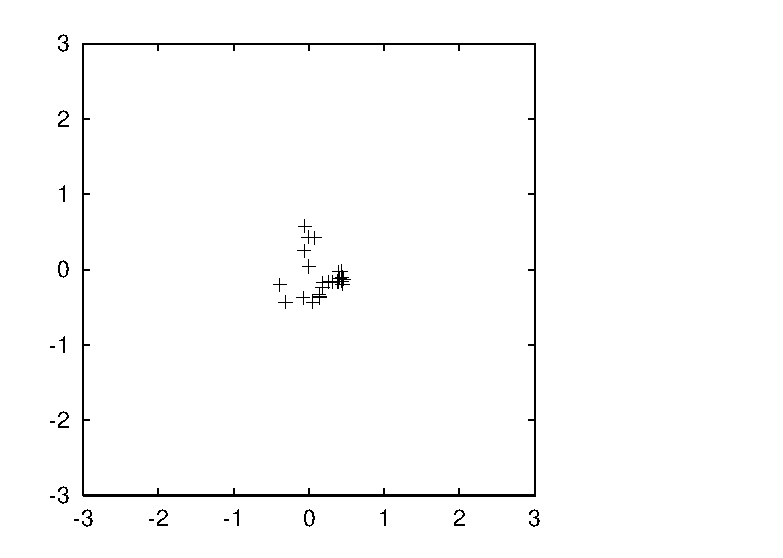
\includegraphics[width=4.5in]{chap10/movietmp_nbody1.out.0.ps}
\caption[1st frame of movie \#1]
{1st frame of the first movie}
\label{fig:movie1.1}
\end{figure}

\begin{figure}[htb]
\centering
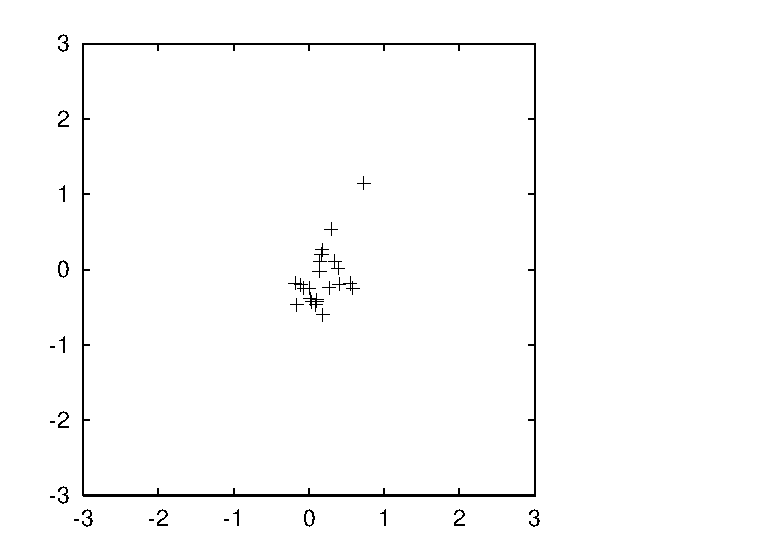
\includegraphics[width=4.5in]{chap10/movietmp_nbody1.out.1.ps}
\caption[2nd frame of movie \#1]
{2nd frame of the first movie}
\label{fig:movie1.2}
\end{figure}

\begin{figure}[htb]
\centering
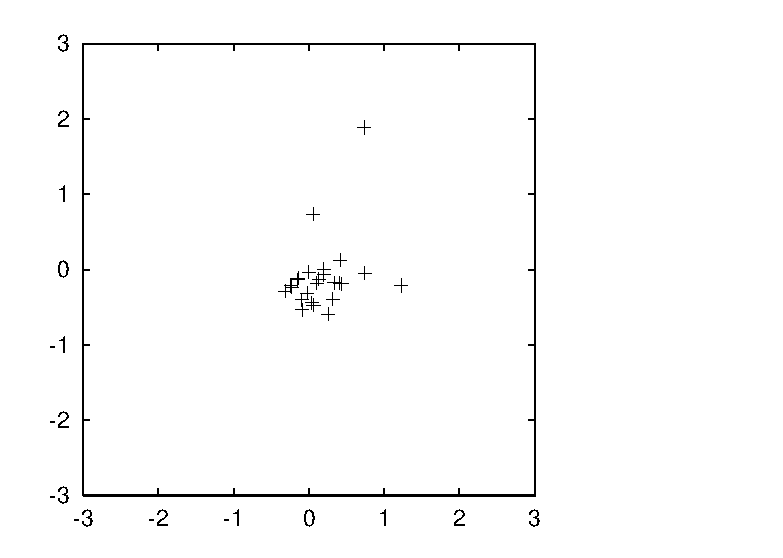
\includegraphics[width=4.5in]{chap10/movietmp_nbody1.out.2.ps}
\caption[3rd frame of movie \#1]
{3rd frame of the first movie}
\label{fig:movie1.3}
\end{figure}

\begin{figure}[htb]
\centering
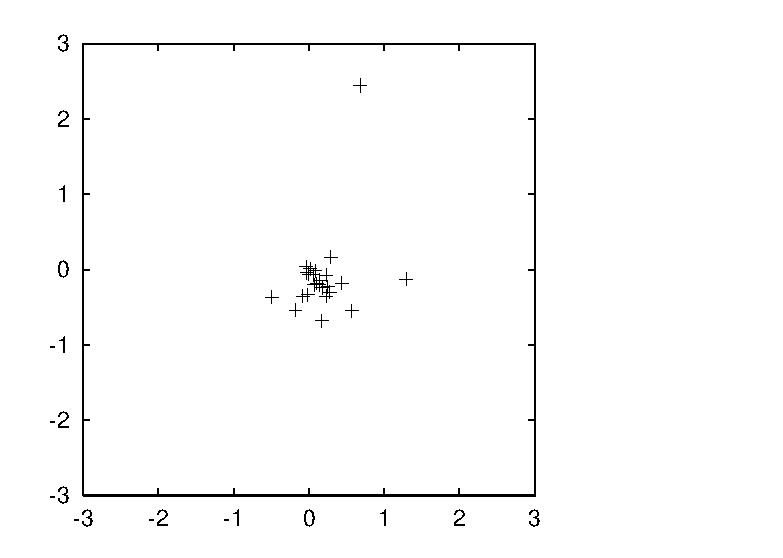
\includegraphics[width=4.5in]{chap10/movietmp_nbody1.out.3.ps}
\caption[4th frame of movie \#1]
{4th frame of the first movie}
\label{fig:movie1.4}
\end{figure}

\begin{figure}[htb]
\centering
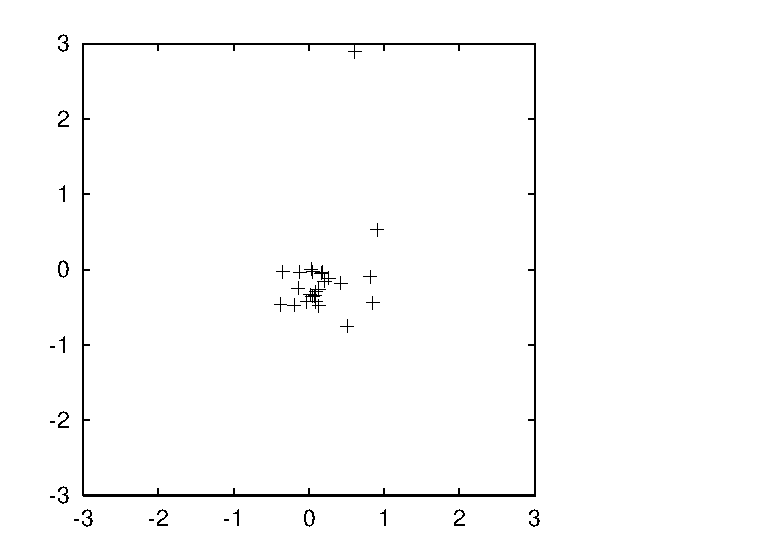
\includegraphics[width=4.5in]{chap10/movietmp_nbody1.out.4.ps}
\caption[5th frame of movie \#1]
{5th frame of the first movie}
\label{fig:movie1.5}
\end{figure}

\begin{figure}[htb]
\centering
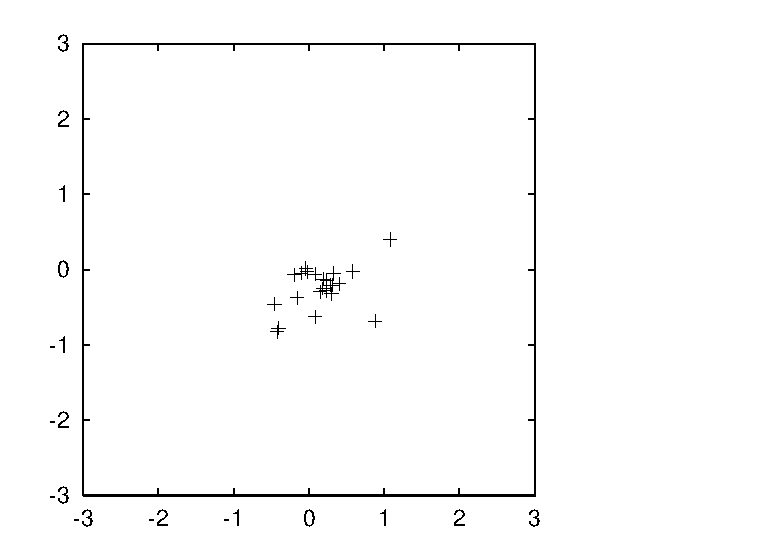
\includegraphics[width=4.5in]{chap10/movietmp_nbody1.out.5.ps}
\caption[6th frame of movie \#1]
{6th frame of the first movie}
\label{fig:movie1.6}
\end{figure}

\begin{figure}[htb]
\centering
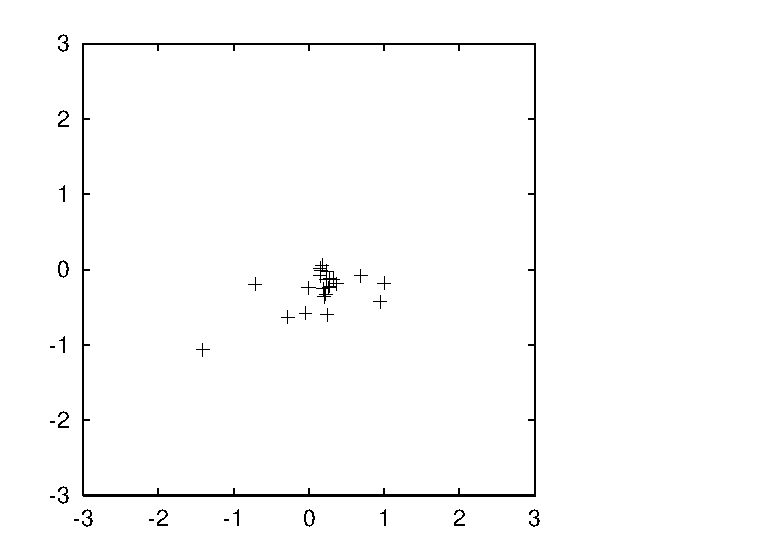
\includegraphics[width=4.5in]{chap10/movietmp_nbody1.out.6.ps}
\caption[7th frame of movie \#1]
{7th frame of the first movie}
\label{fig:movie1.7}
\end{figure}

\begin{figure}[htb]
\centering
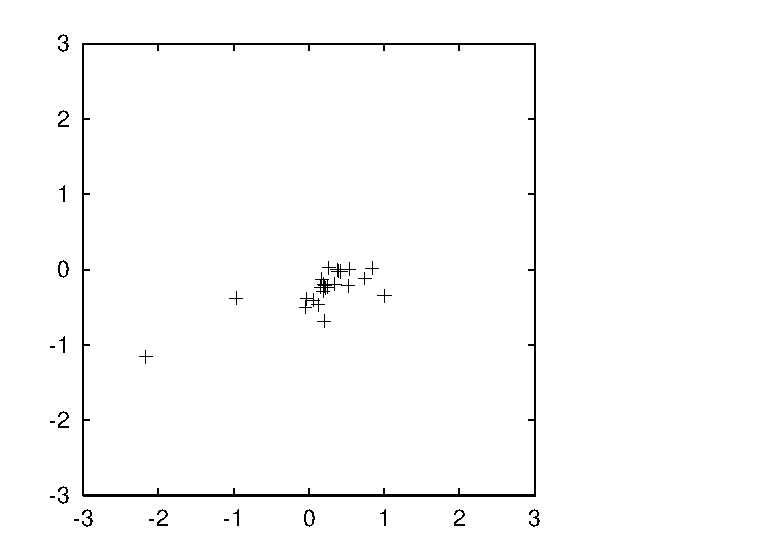
\includegraphics[width=4.5in]{chap10/movietmp_nbody1.out.7.ps}
\caption[8th frame of movie \#1]
{8th frame of the first movie}
\label{fig:movie1.8}
\end{figure}

\begin{figure}[htb]
\centering
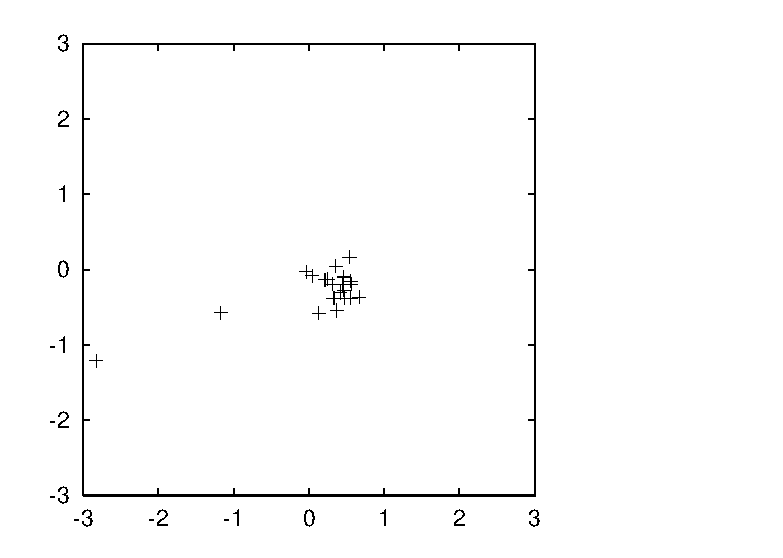
\includegraphics[width=4.5in]{chap10/movietmp_nbody1.out.8.ps}
\caption[9th frame of movie \#1]
{9th frame of the first movie}
\label{fig:movie1.9}
\end{figure}

\begin{figure}[htb]
\centering
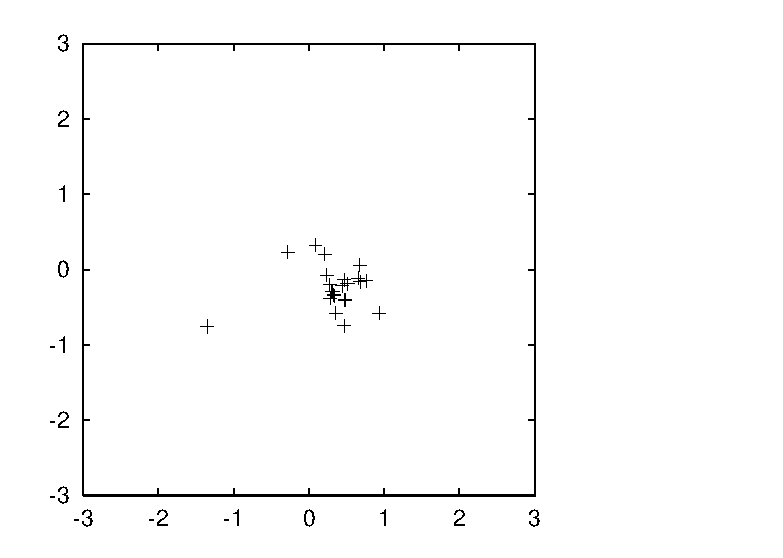
\includegraphics[width=4.5in]{chap10/movietmp_nbody1.out.9.ps}
\caption[10th frame of movie \#1]
{10th frame of the first movie}
\label{fig:movie1.10}
\end{figure}

\clearpage  % to let the ten movie frames be inserted not further than here

\abc

\carol
I guess I passed, yes?  You want my autograph?

\alice
Did you see individual stars escaping?  Real astrophysics going on
here, lady and gentleman!

\bob
Yes, I saw some stars boiling off into deep space, but I must admit, I
couldn't quite follow what was happening in the inner core.  It was
worse than the old slapstick: everything was moving just too fast.

\carol
Lets get ten times as many snapshot frames, but decreasing the output
time intervals from the default of one time unit to one tenth of a
time unit.

\bob
Let's see, right, that was option {\st -o 0.1}, with {\st o} standing
for output interval.  If I work with this code a few more times I'll
get familiar with all the options.  Let's see what happens now.

\cba

\begin{small}
\begin{verbatim}
|gravity> ../chap9/sphere -n 25 | ../chap8/nbody_sh1 -o 0.1 -e 10 > nbody2.out
seed = 1064697607
Starting a Hermite integration for a 25-body system,
  from time t = 0 with time step control parameter dt_param = 0.03  until time 10 ,
  with diagnostics output interval dt_dia = 10,
  and snapshot output interval dt_out = 0.1.
at time t = 0 , after 0 steps :
  E_kin = 0 , E_pot = -0.53095 , E_tot = -0.53095
                absolute energy error: E_tot - E_init = 0
                relative energy error: (E_tot - E_init) / E_init = -0
at time t = 10 , after 102258 steps :
  E_kin = 0.523367 , E_pot = -1.05432 , E_tot = -0.530958
                absolute energy error: E_tot - E_init = -8.39424e-06
                relative energy error: (E_tot - E_init) / E_init = 1.58099e-05
|gravity>
\end{verbatim}
\end{small}

\abc

\carol
Again, a reasonable relative energy, comparable to what we had before.
Now let us follow all those stars step by step.

\cba

\begin{small}
\begin{verbatim}
|gravity> makemovie1.csh nbody2.out
rm: No match.
2 nbody2.out
snapno = 1
snapno = 2
snapno = 3
 . . . .
snapno = 98
snapno = 99
snapno = 100
Hit return to exit
|gravity>
\end{verbatim}
\end{small}

\begin{figure}[htb]
\centering
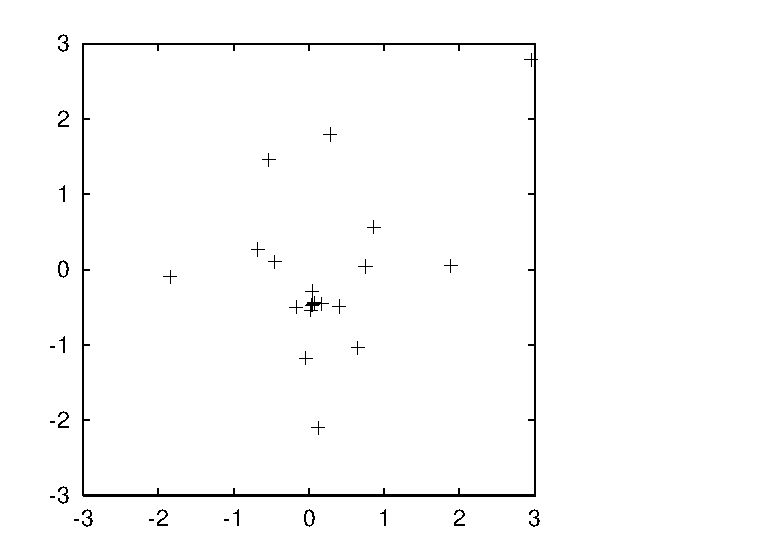
\includegraphics[width=4.5in]{chap10/movie2.ps}
\caption[last frame of movie \#2]
{Last frame of the second movie, from the data stored in {\st nbody2.out}}
\label{fig:movie2}
\end{figure}

\abc

\bob
That's more like it.  Now we can really follow what's going on.

\carol
Well, yes and no.  We can now follow the individual particles all right,
but what about those binaries that Alice had promised us, as the
explanation for the mysterious increase in computer time that we saw
yesterday?

\alice
Well, I'm not sure.  But my guess would be that those binaries are too
small to see easily, on the scale we have plotted them.  After all,
they were so compute expensive exactly because the two stars of such a
binary were bound in a short orbit -- or so we hypothesized.

\bob
Even so, wouldn't we have clearly seen that there were places where
two symbols on the screen almost overlapped?

\carol
I do believe I saw a few cases like that, but I can't be completely
sure.

\alice
The other problem is that binaries are more massive than single stars,
so they tend to sink to the center of a star cluster, where everything
is more crowded.  This is due to equipartition.

\bob
And what is equipartition?

\alice
It is an effect that is similar to what happens with molecules in the air.
Carbon dioxide molecules, for example, are heavier than other
molecules in air, and therefore they tend to stay lower.

\carol
Yes, I remember my high school teacher taking a beaker with carbon dioxide,
which he had obtained from a pressure cylinder.  And then he poured
the invisible gas over a flame, dousing it immediately.  It was very
impressive.

\bob
But how come that carbon dioxide does not fall out of the air?  I
thought it was mixed rather thoroughly in the air around us.

\alice
That's because air currents tend to mix all gases, light or heavy.
Even grass pollen, which are far more heavier than any gas molecule
are carried along with the slightest breeze.

\carol
Tell me all about it.  My allergy season is about to come up again,
which is no fun.

\alice
However, when you carefully pour carbon dioxide, it will stay at the
bottom of a room for a while.  Similarly, a lighter gas, like helium,
will flow up -- which is the reason that a helium balloon indeed rises,
even though the plastic surrounding the helium is heavier than air.

\bob
But what does all that have to do with binaries sinking to the center
of a star cluster?

\alice
The combined gravitational force of all the stars points toward the
center of the cluster.  Heavier `molecules', in our case binaries,
therefore tend to sink to the center, just like carbon dioxide
molecules tend to sink to the floor of a lab.

\carol
All nice and fine, but we're now speculating on and on about binaries,
and we're not yet sure whether we've seen one.  Aren't we running the
danger of discussing how many angles can dance on the tip of a needle?

\bob
In order to dance together, perhaps angles have to form binaries too?

\carol
You're now imagining binaries everywhere.  I want proof.

\alice
I have an idea.  Rather than trying to peer in more and more details
at those movie frames, why not build a binary detector!

\bob
A binary detector?

\alice
Yes!  Just like physicists build elementary particle detectors,
which they use in their accelerators to see what they've got, after
smashing subatomic particles into each other.

\bob
That makes sense.  After all, we have build a star accelerator, in the
form of our $N$-body integrator {\st nbody\_sh1.C}.  Our movie was in
fact a star detector.  So it would be a logical next step to build a
more sophisticated and specialized detector, one that would only be
triggered by binaries.

\carol
That sounds like fun.  But how to go about it?

\alice
The idea is simple.  You just check all possible pairs of particles,
and check to see which ones are bound together, forming a binary.

\carol
That's reasonable, since even with 25 particles, and 100 snapshots,
you only have to check $25*25*100 = 62,500$ pairs, and with so many
millions of floating point operations per second, even on laptops,
that should be no problem.

\bob
After all, at every time step we had to compute the pairwise forces,
which meant 625 pairwise forces far much more often than 100 times in
our run.  So time won't be a problem.  But what type of algorithm
would you use?

\alice
I'm afraid we would have to start with a reasonable amount of
celestial mechanics.  And rather than trying to derive all the
relationships from scratch, let's get together again tomorrow.
I'll bring my celestial mechanics book with me, and then we can
figure it out.

\cba

